\documentclass{article}
%packages
\usepackage{graphicx}
\usepackage[latin1]{inputenc}
\usepackage[T1]{fontenc}
\usepackage[frenchb]{babel}
\usepackage[a4paper]{geometry}
\usepackage{textcomp}
\begin{document}
%title
\begin{titlepage}
	\vspace{-20px}
	\begin{tabular}{l}
		\textsc{Blin} S\'ebastien\\
		\textsc{Collin} Pierre-Henri
	\end{tabular}
	\hfill \vspace{10px}
\includegraphics[scale=0.1]{esir.png}\\
	\vfill
	\begin{center}
		\Huge{\'Ecole sup\'erieure d'ing\'enieurs de Rennes}\\
		\vspace{1cm}
		\LARGE{1\`ere Ann\'ee}\\
		\large{Parcours Informatique}\\
		\vspace{0.5cm}\hrule\vspace{0.5cm}
		\LARGE{\textbf{BDD}}\\
		\Large{Compte-Rendu TP \no 4\textbackslash5\textbackslash6}
		\vspace{0.5cm}\hrule
		\vfill
		\vfill
	\end{center}
	\begin{flushleft}
		\Large{Sous l'encadrement de~:}\\
		\vspace{0.2cm}
		\large{{Zoltan} Miklos}
	\end{flushleft}
	\vfill
\end{titlepage}
\section{Analyse des besoins}
\subsection{\textit{Fonctionnalit\'e essentielle}}
\begin{itemize}
\item Emploi du temps d\textquotesingle un \'etudiant
\item Emploi du temps d\textquotesingle un enseignant
\item Enseignant d'un cours
\item Liste des \'etudiants qui suivent un cours sp\'ecifique
\item Horaires d'un cours
\end{itemize}
\subsection{\textit{Fonctionnalit\'e importante}}
\begin{itemize}
\item Emploi du temps d\textquotesingle un parcours
\item Salles occup\'ees/non-occup\'ees
\end{itemize}
\subsection{\textit{Fonctionnalit\'e utile}}
\begin{itemize}
\item Occupation moyenne des salles
\end{itemize}
\section{Conception du sch\'ema}
Nous avons d\'efini 5 entit\'es (Enseignant, Cours, Salle, Etudiant et Parcours) et 3 associations (Enseigne, estDans et estInscrit) pour r\'ealiser les fonctionnalit\'es essentielles.
\begin{figure}[!h]
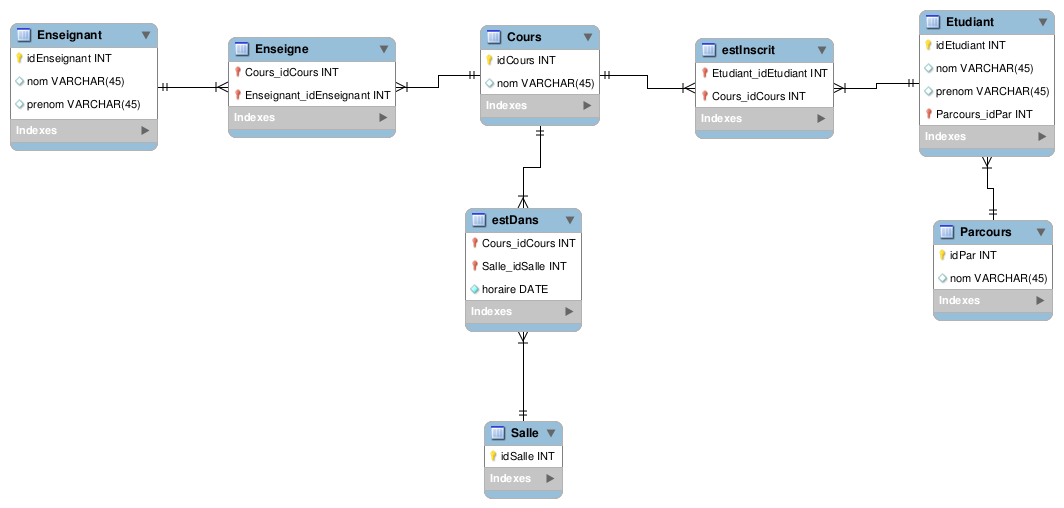
\includegraphics[scale=0.40]{diagramm.png}
\caption{Sch\'ema r\'ealis\'e \`a l\textquotesingle aide de \textit{MySQL Workbench}}
\end{figure}
\section{Quelques requ\^etes}
Voici une liste non-exhaustive de requ\^etes SQL correspondant aux besoins \'enonc\'es ci-dessus :\\
\begin{itemize}
\item Lister l\textquotesingle emploi du temps (d\textquotesingle un cr\'eneau sp\'ecifique) pour un parcours.\\
\begin{verbatim}
SELECT DISTINCT horaire FROM estDans eD, Cours C, estInscrit eI, Etudiant E 
WHERE eD.Cours_idCours=C.idCours 
AND C.idCours=eI.idCours AND eI.idEtudiant=E.idEtudiant AND E.Parcours_idPar=2;

\end{verbatim}
\item Trouver le nom des enseignants pour un cours sp\'ecifique.\\
\begin{verbatim}
SELECT Enseignant_idEnseignant FROM Enseigne WHERE Cours_idCours = 1;

\end{verbatim}
\item Horaires d\textquotesingle un cours sp\'ecifique (par ex. la date du prochain cours de bases de donn\'ees).\\
\begin{verbatim}
SELECT horaire FROM estDans WHERE Cours_idCours = 2;

\end{verbatim}
\item Obtenir une liste des \'etudiants (d\textquotesingle un parcours)\\
\begin{verbatim}
SELECT * FROM Etudiant WHERE Parcours_idPar = 2;

\end{verbatim}
\item Occupation d\textquotesingle une salle sp\'ecifique.\\
\begin{verbatim}
SELECT * FROM estDans WHERE Salle_idSalle = 20;

\end{verbatim}
\item Lister l\textquotesingle emploi du temps (d\textquotesingle un cr\'eneau sp\'ecifique) pour un \'etudiant particulier.\\
\begin{verbatim}
SELECT horaire FROM estDans 
WHERE Cours_idCours = 
(SELECT idCours FROM estInscrit WHERE idEtudiant = 1) AND horaire > '2010';

SELECT horaire FROM estDans 
WHERE Cours_idCours = 
(SELECT idCours FROM estInscrit WHERE idEtudiant = numEtudiant) 
AND horaire > creneau_inf AND horaire < creneau_sup;

\end{verbatim}
\item Lister l\textquotesingle emploi du temps (d\textquotesingle un cr\'eneau sp\'ecifique) pour un enseignant.\\
\begin{verbatim}
SELECT horaire FROM estDans WHERE Cours_idCours = 
(SELECT Cours_idCours FROM Enseigne WHERE Enseignant_idEnseignant = 1)

\end{verbatim}
\item Obtenir une liste des \'etudiants (d\textquotesingle un parcours) qui suivent un cours sp\'ecifique.\\
\begin{verbatim}
SELECT nom, prenom FROM estInscrit EI, Etudiant E 
WHERE  EI.idEtudiant = E.idEtudiant AND E.Parcours_idPar = 1
AND EI.idCours = 1;

\end{verbatim}
\item Liste des salles (de TP/ou autre type) non-occup\'ees (dans une p\'eriode sp\'ecifique)\\
\begin{verbatim}
SELECT DISTINCT Salle_idSalle FROM estDans 
WHERE Salle_idSalle != 
(SELECT DISTINCT Salle_idSalle FROM estDans 
WHERE horaire > '2014' AND horaire < '2016');

\end{verbatim}
\item D\'eterminer l\textquotesingle occupation moyenne des salles de TP.\\
\begin{verbatim}
Soit X le nombre de creneaux sur une periode T. A raison de 8 creneaux par jour. 
Pour une semaine, on a donc X = 40;
SELECT COUNT(horaire)/40 FROM estDans 
WHERE horaire > '2015-05-04' AND horaire < '2015-05-11' AND Salle_idSalle = 1;
SELECT COUNT(horaire)/X FROM estDans 
WHERE horaire > min AND horaire < sup AND Salle_idSalle = salle

\end{verbatim}
\end{itemize}
\section{Interface JDBC}
\subsection{Partie graphique}
L\textquotesingle interface graphique que nous avons d\'evelopp\'e est compos\'ee de deux parties :
\begin{itemize}
\item Une rang\'ee de boutons qui permettent de se connecter \`a la base de donn\'ees, de se d\'econnecter, et d\textquotesingle envoyer des requ\^etes en fonction de ce que l'utilisateur souhaite obtenir comme information. Ainsi, il peut obtenir la liste de tous les enseignants, des \'etudiants, des horaires de cours, des horaires de parcours et des salles. 
\item Un ensemble de zones de texte qui permettent de filtrer les r\'esultats et d'obtenir une recherche plus affin\'ee. Par exemple, lorsque qu\textquotesingle on souhaite conna\^itre les horaires d'un cours, on pr\'ecise le num\'ero du cours dans le champ correspondant.\\
\end{itemize} 
\begin{figure}[!h]
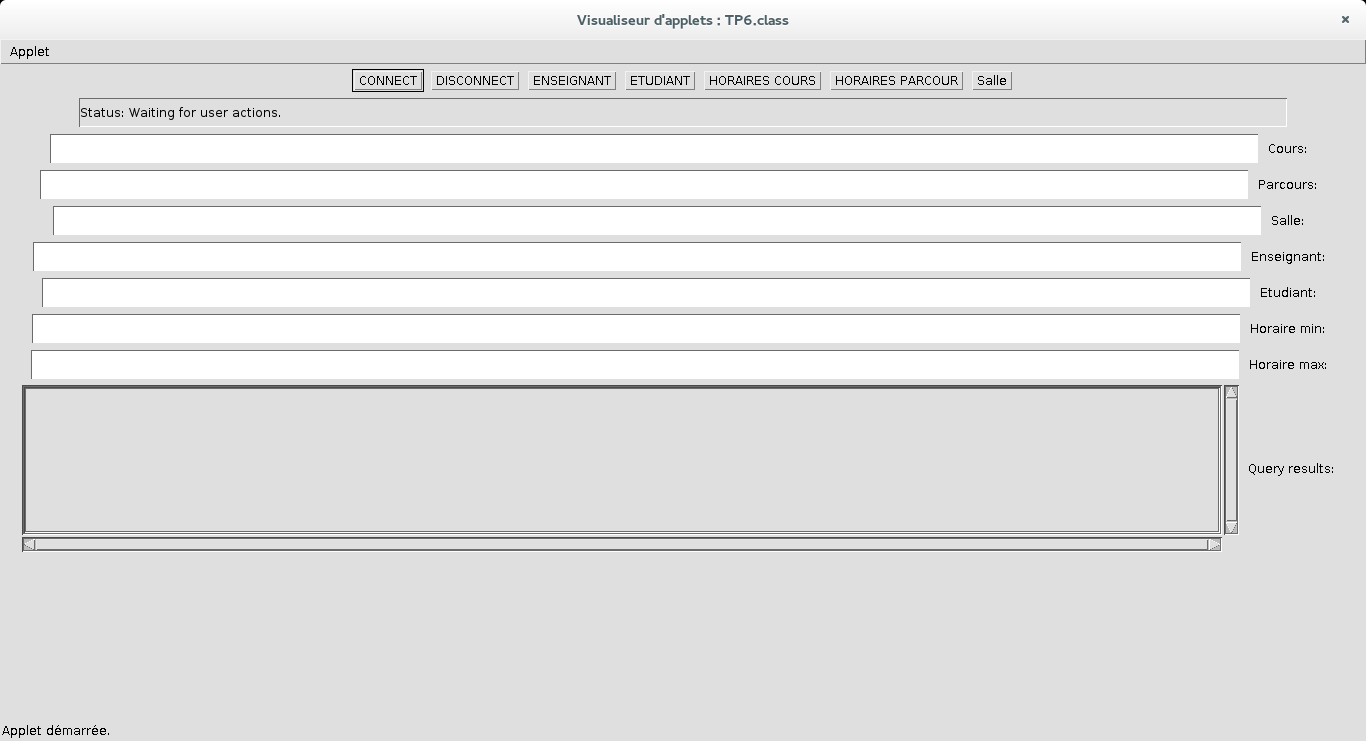
\includegraphics[scale=0.33]{applet.png}
\caption{Aper\c{c}u de l\textquotesingle applet}
\end{figure}
\subsection{Code source}
\begin{verbatim}

import java.awt.*;
import java.awt.event.*;
import java.sql.*;

/**
 * This is a skeleton for realizing a very simple database user interface in java. 
 * The interface is an Applet, and it implements the interface ActionListener. 
 * If the user performs an action (for example he presses a button), the procedure actionPerformed 
 * is called. Depending on his actions, one can implement the database connection (disconnection), 
 * querying or insert. 
 * 
 * @author zmiklos
 *
 */
public class TP6 extends java.applet.Applet implements ActionListener {

 private TextField mStat, mCours, mParcours, mSalle, 
 mEnseignant, mEtudiant, mHoraireMin, mHoraireMax;
 TextArea mRes;
 private Button b1, b2, bEnseignant, bEtudiant,
 bHoraireCours, bHoraireParcours, bSalle;
 private static final long serialVersionUID = 1L; 
 
 // JDBC driver name and database URL
   static final String JDBC_DRIVER = "com.mysql.jdbc.Driver";  
   static final String DB_URL = "jdbc:mysql://mysql.istic.univ-rennes1.fr:3306/base_13002155";

   //  Database credentials
   static final String USER = "user_13002155";
   static final String PASS = "lolgithub";  
   
		Connection conn = null;
		Statement stmt = null;
 
 
 /**
  * This procedure is called when the Applet is initialized.
  * 
  */
 public void init ()
 {    
	 /**
	  * Definition of text fields
	  */
     mStat = new TextField(150);
     mStat.setEditable(false);
     mRes = new TextArea(10,150);
     mRes.setEditable(false);
     mCours = new TextField(150);
     mParcours = new TextField(150);
     mSalle = new TextField(150);
     mEnseignant = new TextField(150);
     mEtudiant= new TextField(150);
     mHoraireMin = new TextField(150);
     mHoraireMax = new TextField(150);
    
     
     
     /**
      * First we define the buttons, then we add to the Applet, 
      * finally add and ActionListener 
      * (with a self-reference) to capture the user actions.  
      */
     b1 = new Button("CONNECT");
     b2 = new Button("DISCONNECT");
     bEnseignant = new Button("ENSEIGNANT");
     bEtudiant = new Button("ETUDIANT");
     bHoraireCours = new Button("HORAIRES COURS");
     bHoraireParcours = new Button("HORAIRES PARCOUR");
     bSalle = new Button("Salle");
     add(b1) ;
     add(b2) ;
     add(bEnseignant) ;
     add(bEtudiant) ;
     add(bHoraireCours);
     add(bHoraireParcours);
     add(bSalle);
     b1.addActionListener(this);
     b2.addActionListener(this);
     bEnseignant.addActionListener(this);
     bEtudiant.addActionListener(this);
     bHoraireCours.addActionListener(this);
     bHoraireParcours.addActionListener(this);
     bSalle.addActionListener(this);
     
     
     add(mStat);
     setLayout(new FlowLayout());
     add(mCours);
     add(new Label("Cours: ",Label.CENTER));
     add(mParcours);
     add(new Label("Parcours: ", Label.CENTER));
     add(mSalle);
     add(new Label("Salle: ", Label.CENTER));
     add(mEnseignant);
     add(new Label("Enseignant: ", Label.CENTER));
     add(mEtudiant);
     add(new Label("Etudiant: ", Label.CENTER));
     add(mHoraireMin);
     add(new Label("Horaire min: ", Label.CENTER));
     add(mHoraireMax);
     add(new Label("Horaire max: ", Label.CENTER));
     add(mRes);
     add(new Label("Query results: ", Label.CENTER));
     
     
     setStatus("Waiting for user actions.");
 }
 
 
 /**
  * This procedure is called upon a user action.
  * 
  *  @param event The user event. 
  */
  public void actionPerformed(ActionEvent event)
 {
  
	 // Extract the relevant information from the action 
	 // (i.e. which button is pressed?)
	 Object cause = event.getSource();

	 // Act depending on the user action
	 // Button CONNECT
     if (cause == b1)
     {
        connectToDatabase();
     }
     
     // Button DISCONNECT
     if (cause == b2)
     {
    	 disconnectFromDatabase();
     }
     
     if (cause == bEnseignant)
     {
    	 QueryEnseignant();
     }
     
     if (cause == bEtudiant)
     {
    	 QueryEtudiant();
     }
     
     if (cause == bHoraireCours)
     {
    	 QueryHoraireCours();
     }
     
     if (cause == bHoraireParcours)
     {
    	 QueryHoraireParcours();
     }

     if (cause == bSalle)
     {
    	 QuerySalle();
     }
 }
 

/**
 * Set the status text. 
 * 
 * @param text The text to set. 
 */
private void setStatus(String text){
	    mStat.setText("Status: " + text);
  }

/**
 * Procedure, where the database connection should be implemented. 
 */
private void connectToDatabase(){
	try{
		//STEP 2: Register JDBC driver
		Class.forName("com.mysql.jdbc.Driver");

		//STEP 3: Open a connection
		System.out.println("Connecting to database...");
		conn = DriverManager.getConnection(DB_URL,USER,PASS);
		if(conn != null)
			setStatus("Connected to the database");
	} catch(Exception e){
		System.err.println(e.getMessage());
		setStatus("Connection failed" + e.toString());
	}
}


/**
 * Procedure, where the database connection should be implemented. 
 */
private void disconnectFromDatabase(){
	try{
	setStatus("Disconnected from the database");
	} catch(Exception e){
        if(conn!=null)
			try {
				conn.close();
			} catch (SQLException e1) {
				e1.printStackTrace();
			}
		System.err.println(e.getMessage());
		setStatus("Disconnection failed");
	}
}

/**
 * Search Enseignant in Enseigne 
 */
private void QueryEnseignant(){
	try{
		stmt = conn.createStatement();
	    String sql;
	    sql = "SELECT prenom, nom FROM Enseigne as E, Enseignant 
	    WHERE Enseignant.idEnseignant = E.Enseignant_idEnseignant";
	    if(!mCours.getText().isEmpty())
	    	sql += " AND Cours_idCours = " + mCours.getText();
	    System.out.println(sql);
	    ResultSet rs = stmt.executeQuery(sql);
	    mRes.setText("");
	    //STEP 5: Extract data from result set
	    while(rs.next()){
	       //Retrieve by column name
	       String prenom = rs.getString("prenom");
	       String nom = rs.getString("nom");
	
	       //Display values
	       
	       mRes.append("Enseignant: " + nom + " " + prenom + "\n");
	    }
	    
	    stmt.close();
	    rs.close();
	} catch(Exception e){
			System.err.println(e.getMessage());
			setStatus("Requete ratee");
		}
	
}

/**
 * Recherche un etudiant
 */
private void QueryEtudiant(){
	try{
		stmt = conn.createStatement();
	    String sql;
	    sql = "SELECT nom, prenom FROM estInscrit EI, Etudiant E 
	    WHERE  EI.idEtudiant = E.idEtudiant";
	    if(!mParcours.getText().isEmpty())
	    	sql += " And E.Parcours_idPar = " + mParcours.getText();
	    if(!mCours.getText().isEmpty())
	    	sql += " And EI.idCours = " + mCours.getText();
	    System.out.println(sql);
	    ResultSet rs = stmt.executeQuery(sql);
	    //mRes.setText("");
	    //STEP 5: Extract data from result set
	    while(rs.next()){
	       //Retrieve by column name
	       String prenom = rs.getString("prenom");
	       String nom = rs.getString("nom");
	
	       //Display values
	       
	       mRes.append("Etudiant: " + nom + " " + prenom + "\n");
	    }
	    
	    stmt.close();
	    rs.close();
	} catch(Exception e){
			System.err.println(e.getMessage());
			setStatus("Requete ratee");
		}
	
}


/**
 * Horaire
 */
private void QueryHoraireCours(){
	try{
		stmt = conn.createStatement();
	    String sql;
	    sql = "SELECT * FROM estDans WHERE";
	    System.out.println(sql);
	    if(!mCours.getText().isEmpty())
	    	sql += " Cours_idCours= " + mCours.getText();
	    else if(!mEnseignant.getText().isEmpty())
	    	sql += " Cours_idCours = (SELECT Cours_idCours 
	    	FROM Enseigne 
	    	WHERE Enseignant_idEnseignant = "+mEnseignant.getText()+")";
	    else if(!mEtudiant.getText().isEmpty())
	    	sql += " Cours_idCours = (SELECT idCours 
	    	FROM estInscrit 
	    	WHERE idEtudiant= "+mEtudiant.getText()+")";
	    else
	    	sql += " Salle_idSalle = " + mSalle.getText();
	    
	    if(!mHoraireMax.getText().isEmpty() && !mHoraireMin.getText().isEmpty())
	    	sql += "AND horaire > '"+mHoraireMin.getText()+"' 
	    	AND horaire < '"+mHoraireMax.getText()+"'";
	    System.out.println(sql);
	    ResultSet rs = stmt.executeQuery(sql);
	    mRes.setText("");
	    //STEP 5: Extract data from result set
	    while(rs.next()){
	       //Retrieve by column name
		   String cours = rs.getString("Cours_idCours");
		   String salle = rs.getString("Salle_idSalle");
	       String horaire = rs.getString("horaire");
	
	       //Display values
	       
	       mRes.append("Horaire: " + cours + "-" + salle + "-" + horaire + "\n");
	    }
	    
	    stmt.close();
	    rs.close();
	} catch(Exception e){
			System.err.println(e.getMessage());
			setStatus("Requete ratee");
		}
	
}

/**
 * Horaire
 */
private void QueryHoraireParcours(){
	try{
		stmt = conn.createStatement();
	    String sql;
	    sql = "SELECT DISTINCT horaire FROM estDans eD, Cours C, estInscrit eI, Etudiant E 
	    		WHERE eD.Cours_idCours=C.idCours AND C.idCours=eI.idCours 
	    		AND eI.idEtudiant=E.idEtudiant AND E.Parcours_idPar=" + mParcours.getText();
	    System.out.println(sql);
	    ResultSet rs = stmt.executeQuery(sql);
	    mRes.setText("");
	    //STEP 5: Extract data from result set
	    while(rs.next()){
	       //Retrieve by column name
	       String horaire = rs.getString("horaire");
	
	       //Display values
	       
	       mRes.append("Horaire: " + horaire + "\n");
	    }
	    
	    stmt.close();
	    rs.close();
	} catch(Exception e){
			System.err.println(e.getMessage());
			setStatus("Requete ratee");
		}
	
}

/**
 * Salle
 */
private void QuerySalle(){
	try{
		stmt = conn.createStatement();
	    String sql;
	    sql = "SELECT DISTINCT Salle_idSalle FROM estDans ";
	    if(!mHoraireMax.getText().isEmpty() && !mHoraireMin.getText().isEmpty())
	    	sql += "WHERE horaire > '"+mHoraireMin.getText()+"' AND horaire < '"
	    	+ mHoraireMax.getText()+"'";
	    System.out.println(sql);
	    ResultSet rs = stmt.executeQuery(sql);
	    mRes.setText("");
	    //STEP 5: Extract data from result set
	    while(rs.next()){
	       //Retrieve by column name
	       String Salle = rs.getString("Salle_idSalle");
	
	       //Display values
	       
	       mRes.append("Salle: " + Salle + "\n");
	    }
	    
	    stmt.close();
	    rs.close();
	} catch(Exception e){
			System.err.println(e.getMessage());
			setStatus("Requete ratee");
		}
	
}


}

\end{verbatim}
\end{document}

